\documentclass[11pt,a4paper]{report}
\usepackage[textwidth=37em,vmargin=30mm]{geometry}
\usepackage{calc,xunicode,amsmath,amssymb,paralist,enumitem,tabu,booktabs,datetime2,xeCJK,xeCJKfntef,listings}
\usepackage{tocloft,fancyhdr,tcolorbox,xcolor,graphicx,eso-pic,xltxtra,xelatexemoji}

\newcommand{\envyear}[0]{2025}
\newcommand{\envdatestr}[0]{2025-10-24}
\newcommand{\envfinaldir}[0]{webdb/2025/20251024/final}

\usepackage[hidelinks]{hyperref}
\hypersetup{
    colorlinks=false,
    pdfpagemode=FullScreen,
    pdftitle={Web Digest - \envdatestr}
}

\setlength{\cftbeforechapskip}{10pt}
\renewcommand{\cftchapfont}{\rmfamily\bfseries\large\raggedright}
\setlength{\cftbeforesecskip}{2pt}
\renewcommand{\cftsecfont}{\sffamily\small\raggedright}

\setdefaultleftmargin{2em}{2em}{1em}{1em}{1em}{1em}

\usepackage{xeCJK,xeCJKfntef}
\xeCJKsetup{PunctStyle=plain,RubberPunctSkip=false,CJKglue=\strut\hskip 0pt plus 0.1em minus 0.05em,CJKecglue=\strut\hskip 0.22em plus 0.2em}
\XeTeXlinebreaklocale "zh"
\XeTeXlinebreakskip = 0pt


\setmainfont{Brygada 1918}
\setromanfont{Brygada 1918}
\setsansfont{IBM Plex Sans}
\setmonofont{JetBrains Mono NL}
\setCJKmainfont{Noto Serif CJK SC}
\setCJKromanfont{Noto Serif CJK SC}
\setCJKsansfont{Noto Sans CJK SC}
\setCJKmonofont{Noto Sans CJK SC}

\setlength{\parindent}{0pt}
\setlength{\parskip}{8pt}
\linespread{1.15}

\lstset{
	basicstyle=\ttfamily\footnotesize,
	numbersep=5pt,
	backgroundcolor=\color{black!5},
	showspaces=false,
	showstringspaces=false,
	showtabs=false,
	tabsize=2,
	captionpos=b,
	breaklines=true,
	breakatwhitespace=true,
	breakautoindent=true,
	linewidth=\textwidth
}






\newcommand{\coverpic}[2]{
    % argv: itemurl, authorname
    Cover photo by #2~~(\href{#1}{#1})
}
\newcommand{\makeheader}[0]{
    \begin{titlepage}
        % \newgeometry{hmargin=15mm,tmargin=21mm,bmargin=12mm}
        \begin{center}
            
            \rmfamily\scshape
            \fontspec{BaskervilleF}
            \fontspec{Old Standard}
            \fontsize{59pt}{70pt}\selectfont
            WEB\hfill DIGEST
            
            \vfill
            % \vskip 30pt
            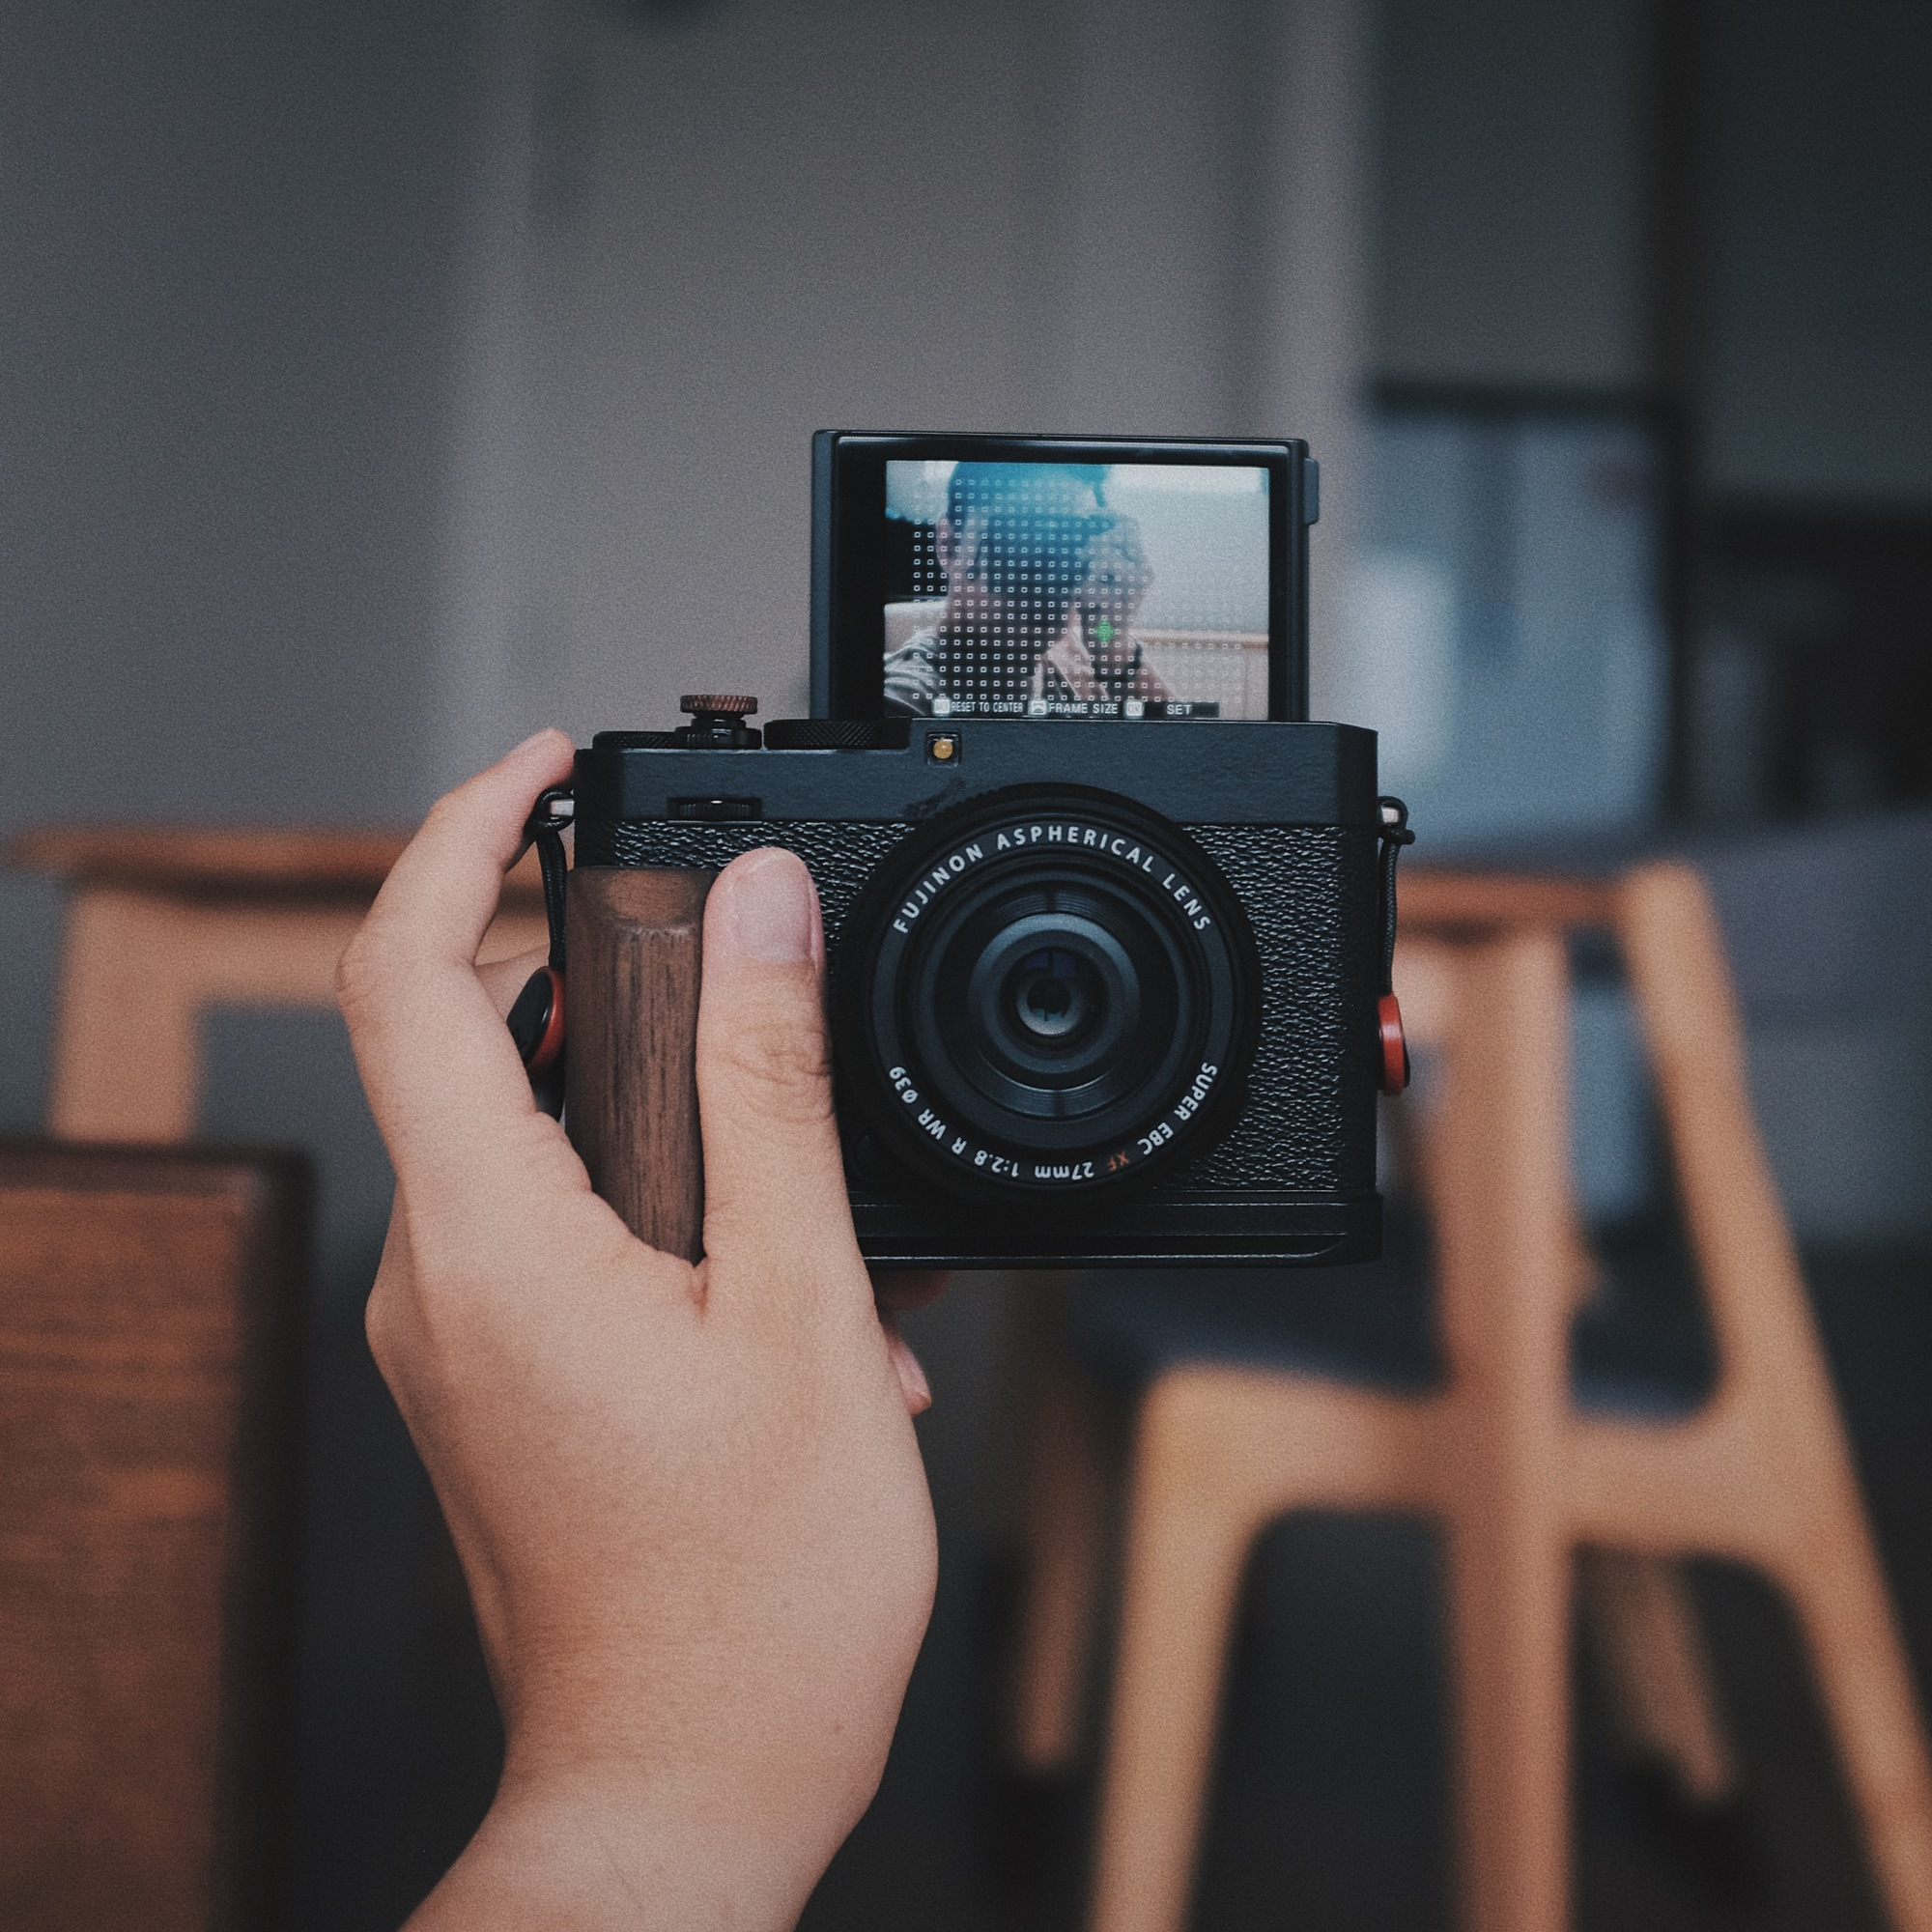
\includegraphics[width=\linewidth]{\envfinaldir/coverpic-prod.jpg}\par
            % \vskip 30pt
            \vfill

            \normalsize\rmfamily\scshape
            \copyright{} The Web Digest Project \hfill\large \envdatestr
        \end{center}
    \end{titlepage}
    % \restoregeometry
}
\newcommand{\simplehref}[1]{%
    \textcolor{blue!80!green}{\href{#1}{#1}}%
}
\renewcommand{\contentsname}{\center\Huge\sffamily\bfseries Contents\par\vskip 20pt}
\newcounter{ipartcounter}
\setcounter{ipartcounter}{0}
\newcommand{\ipart}[1]{
    % \vskip 20pt
    \clearpage
    \stepcounter{ipartcounter}
    \phantomsection
    \addcontentsline{toc}{chapter}{#1}
    % \begin{center}
    %     \Huge
    %     \sffamily\bfseries
    %     #1
    % \end{center}
    % \vskip 20pt plus 7pt
}
\newcounter{ichaptercounter}
\setcounter{ichaptercounter}{0}
\newcommand{\ichapter}[1]{
    % \vskip 20pt
    \clearpage
    \stepcounter{ichaptercounter}
    \phantomsection
    \addcontentsline{toc}{section}{\numberline{\arabic{ichaptercounter}}#1}
    \begin{center}
        \Huge
        \sffamily\bfseries
        #1
    \end{center}
    \vskip 20pt plus 7pt
}
\newcommand{\entrytitlefont}[1]{\subsection*{\raggedright\Large\sffamily\bfseries#1}}
\newcommand{\entryitemGeneric}[2]{
    % argv: title, url
    \parbox{\linewidth}{
        \entrytitlefont{#1}\par\vskip 5pt
        \footnotesize\ttfamily\mdseries
        \simplehref{#2}
    }\vskip 11pt plus 11pt minus 1pt
}
\newcommand{\entryitemGithub}[3]{
    % argv: title, url, desc
    \parbox{\linewidth}{
        \entrytitlefont{#1}\par\vskip 5pt
        \footnotesize\ttfamily\mdseries
        \simplehref{#2}\par\vskip 5pt
        \small\rmfamily\mdseries#3
    }\vskip 11pt plus 11pt minus 1pt
}
\newcommand{\entryitemAp}[3]{
    % argv: title, url, desc
    \parbox{\linewidth}{
        \entrytitlefont{#1}\par\vskip 5pt
        \footnotesize\ttfamily\mdseries
        \simplehref{#2}\par\vskip 5pt
        \small\rmfamily\mdseries#3
    }\vskip 11pt plus 11pt minus 1pt
}
\newcommand{\entryitemHackernews}[3]{
    % argv: title, hnurl, rawurl
    % \parbox{\linewidth}{
    %     \entrytitlefont{#1}\par\vskip 5pt
    %     \footnotesize\ttfamily\mdseries
    %     \simplehref{#3}\par
    %     \textcolor{black!50}{\href{#2}{#2}}
    % }\vskip 11pt plus 11pt minus 1pt
    \begin{minipage}{\linewidth}
            \entrytitlefont{#1}\par\vskip 5pt
            \footnotesize\ttfamily\mdseries
            \simplehref{#3}\par
            \textcolor{black!50}{\href{#2}{#2}}
    \end{minipage}\par\vskip 11pt plus 11pt minus 1pt
}







\begin{document}

\makeheader

\tableofcontents\clearpage




\ipart{Developers}
\ichapter{Hacker News}
\entryitemTwoLinks{Apple loses UK App Store monopoly case, penalty might near \$2B}{https://news.ycombinator.com/item?id=45688006}{https://9to5mac.com/2025/10/23/apple-loses-uk-app-store-monopoly-case-penalty-might-near-2-billion/}

\entryitemTwoLinks{FocusTube: A Chrome extension that hides YouTube Shorts}{https://news.ycombinator.com/item?id=45687227}{https://github.com/CaptainYouz/FocusTube}

\entryitemTwoLinks{Date bug in Rust-based coreutils affects Ubuntu 25.10 automatic updates}{https://news.ycombinator.com/item?id=45686919}{https://lwn.net/Articles/1043103/}

\entryitemTwoLinks{What happened to Apple's legendary attention to detail?}{https://news.ycombinator.com/item?id=45685551}{https://blog.johnozbay.com/what-happened-to-apples-attention-to-detail.html}

\entryitemTwoLinks{Armed police swarm student after AI mistakes bag of Doritos for a weapon}{https://news.ycombinator.com/item?id=45684934}{https://www.dexerto.com/entertainment/armed-police-swarm-student-after-ai-mistakes-bag-of-doritos-for-a-weapon-3273512/}

\entryitemTwoLinks{OpenMaxIO: Forked UI for MinIO Object Storage}{https://news.ycombinator.com/item?id=45684736}{https://github.com/OpenMaxIO/openmaxio-object-browser}

\entryitemTwoLinks{Show HN: I built a tech news aggregator that works the way my brain does}{https://news.ycombinator.com/item?id=45684689}{https://deadstack.net/recent}

\entryitemTwoLinks{OpenAI acquires Sky.app}{https://news.ycombinator.com/item?id=45684236}{https://openai.com/index/openai-acquires-software-applications-incorporated}

\entryitemTwoLinks{New updates and more access to Google Earth AI}{https://news.ycombinator.com/item?id=45684155}{https://blog.google/technology/research/new-updates-and-more-access-to-google-earth-ai/}

\entryitemTwoLinks{Claude Memory}{https://news.ycombinator.com/item?id=45684134}{https://www.anthropic.com/news/memory}

\entryitemTwoLinks{MinIO declines to release Docker builds resolving CVE-2025-62506}{https://news.ycombinator.com/item?id=45684035}{https://github.com/minio/minio/issues/21647}

\entryitemTwoLinks{Trump pardons convicted Binance founder}{https://news.ycombinator.com/item?id=45683152}{https://www.wsj.com/finance/currencies/trump-pardons-convicted-binance-founder-7509bd63}

\entryitemTwoLinks{US hits \$38T in debt. Fastest accumulation of \$1T outside pandemic}{https://news.ycombinator.com/item?id=45682671}{https://apnews.com/article/trump-treasury-debt-ceiling-bessent-09575f13ca95c2f1beb38234b2cbe85b}

\entryitemTwoLinks{US axes website for reporting human rights abuses by US-armed foreign forces}{https://news.ycombinator.com/item?id=45682169}{https://www.bbc.com/news/articles/cqx30vnwd4do}

\entryitemTwoLinks{I spent a year making an ASN.1 compiler in D}{https://news.ycombinator.com/item?id=45681200}{https://bradley.chatha.dev/blog/dlang-propaganda/asn1-compiler-in-d/}

\entryitemTwoLinks{Show HN: Deta Surf – An open source and local-first AI notebook}{https://news.ycombinator.com/item?id=45680937}{https://github.com/deta/surf}

\entryitemTwoLinks{The game theory of how algorithms can drive up prices}{https://news.ycombinator.com/item?id=45680695}{https://www.quantamagazine.org/the-game-theory-of-how-algorithms-can-drive-up-prices-20251022/}

\entryitemTwoLinks{SpaceX disables 2,500 Starlink terminals allegedly used by Asian scam centers}{https://news.ycombinator.com/item?id=45680547}{https://arstechnica.com/tech-policy/2025/10/starlink-blocks-2500-dishes-allegedly-used-by-myanmars-notorious-scam-centers/}

\entryitemTwoLinks{PyTorch Monarch}{https://news.ycombinator.com/item?id=45680237}{https://pytorch.org/blog/introducing-pytorch-monarch/}

\entryitemTwoLinks{C64 Blood Money}{https://news.ycombinator.com/item?id=45679638}{https://lemmings.info/c64-blood-money/}\ichapter{Phoronix}
\entryitemGeneric{\hskip 0pt{}AMD Radeon AI PRO R9700 Hitting Retailers Next Week For \$1299 USD}{https://www.phoronix.com/news/AMD-Radeon-AI-PRO-R9700-1299}

\entryitemGeneric{\hskip 0pt{}KDE Plasma 6.5's Overlay Planes Support Yields Significant Power Savings}{https://www.phoronix.com/news/Plasma-6.5-Overlay-Planes-KWin}

\entryitemGeneric{\hskip 0pt{}Linux's Proposed Cache Aware Scheduling Benchmarks Show Big Potential On AMD EPYC Turin}{https://www.phoronix.com/review/cache-aware-scheduling-amd-turin}

\entryitemGeneric{\hskip 0pt{}Canonical Academy Announced For New Ubuntu Linux Certifications}{https://www.phoronix.com/news/Canonical-Academy}

\entryitemGeneric{\hskip 0pt{}Ubuntu 25.10 Unattended Upgrades Broken Due To Rust Coreutils Bug}{https://www.phoronix.com/news/Ubuntu-25.10-Broken-Upgrade}

\entryitemGeneric{\hskip 0pt{}Canonical Begins Snap'ing Up Silicon-Optimized AI LLMs For Ubuntu Linux}{https://www.phoronix.com/news/Ubuntu-Snap-Optimized-LLMs}

\entryitemGeneric{\hskip 0pt{}GTK 4.22 To Natively Support SVG - Including Animations}{https://www.phoronix.com/news/GTK-4.22-Native-SVG}

\entryitemGeneric{\hskip 0pt{}ESWIN Launching EBC7702 Mini-DTX RISC-V Board With Dual-Die EIC7702X SoC}{https://www.phoronix.com/news/ESWIN-EBC7702-Mini-DTX-RISC-V}

\entryitemGeneric{\hskip 0pt{}Linux Looks To Orphan Its ISDN Subsystem}{https://www.phoronix.com/news/Linux-2025-Orphan-ISDN-mISDN}


\ipart{Developers~~~~(zh-Hans)}
\ichapter{Solidot}
\entryitemGeneric{\hskip 0pt{}Fedora 批准使用 AI 的政策}{https://www.solidot.org/story?sid=82622}

\entryitemGeneric{\hskip 0pt{}NVIDIA 中国开发者日 2025 将于11月14日在苏州举办}{https://www.solidot.org/story?sid=82620}

\entryitemGeneric{\hskip 0pt{}Google 称其量子计算机首次实现了可验证的量子优势}{https://www.solidot.org/story?sid=82619}

\entryitemGeneric{\hskip 0pt{}AWS 宕机事故导致智能床垫故障}{https://www.solidot.org/story?sid=82618}

\entryitemGeneric{\hskip 0pt{}SpaceX 禁用了缅甸电诈园区逾 2500 个Starlink 终端}{https://www.solidot.org/story?sid=82617}

\entryitemGeneric{\hskip 0pt{}Meta AI 部门裁员 600 人}{https://www.solidot.org/story?sid=82616}

\entryitemGeneric{\hskip 0pt{}VST 3 在 MIT 许可证下开源}{https://www.solidot.org/story?sid=82615}

\entryitemGeneric{\hskip 0pt{}新德里空气污染水平创五年新高}{https://www.solidot.org/story?sid=82614}

\entryitemGeneric{\hskip 0pt{}新癌症疗法利用 LED 和锡纳米片杀死癌细胞}{https://www.solidot.org/story?sid=82613}

\entryitemGeneric{\hskip 0pt{}AI 助手在 45\% 的时间里曲解新闻内容}{https://www.solidot.org/story?sid=82612}

\entryitemGeneric{\hskip 0pt{}每周一到两天步行逾 4 千步与老年女性更低的心脏病和死亡风险相关}{https://www.solidot.org/story?sid=82611}

\entryitemGeneric{\hskip 0pt{}DigiKam 8.8.0 释出}{https://www.solidot.org/story?sid=82610}

\entryitemGeneric{\hskip 0pt{}2024 年全球煤炭消耗创历史新高}{https://www.solidot.org/story?sid=82609}

\entryitemGeneric{\hskip 0pt{}马斯克对 NASA 代理局长宣战}{https://www.solidot.org/story?sid=82608}

\entryitemGeneric{\hskip 0pt{}Valkey 9.0.0 释出}{https://www.solidot.org/story?sid=82607}

\entryitemGeneric{\hskip 0pt{}外国黑客利用 SharePoint 漏洞入侵美国核武器工厂}{https://www.solidot.org/story?sid=82606}

\entryitemGeneric{\hskip 0pt{}OpenAI 发布 AI 浏览器 ChatGPT Atlas}{https://www.solidot.org/story?sid=82605}

\entryitemGeneric{\hskip 0pt{}美国缩小 10 万美元 H-1B 签证费适用范围}{https://www.solidot.org/story?sid=82604}

\entryitemGeneric{\hskip 0pt{}PRIMA 芯片助黄斑变性失明患者恢复视力}{https://www.solidot.org/story?sid=82603}

\entryitemGeneric{\hskip 0pt{}TikTok 修改政策不再提前通知用户政府索要其数据}{https://www.solidot.org/story?sid=82602}\ichapter{V2EX}
\entryitemGeneric{\hskip 0pt{}[VXNA] 申请收录个人博客 https://blog.qiyuor2.me}{https://www.v2ex.com/t/1168011}

\entryitemGeneric{\hskip 0pt{}[Android] 安卓使用一周后感受}{https://www.v2ex.com/t/1168010}

\entryitemGeneric{\hskip 0pt{}[问与答] codex 真的是无语了}{https://www.v2ex.com/t/1168009}

\entryitemGeneric{\hskip 0pt{}[生活] 1024 节快乐~}{https://www.v2ex.com/t/1168008}

\entryitemGeneric{\hskip 0pt{}[NAS] 问问现在组 nas 该选什么}{https://www.v2ex.com/t/1168007}

\entryitemGeneric{\hskip 0pt{}[Go 编程语言] 为什么不用 gRPC-Go: VictoriaTraces 中实现 OTLP/gRPC 的幕后故事}{https://www.v2ex.com/t/1168006}

\entryitemGeneric{\hskip 0pt{}[NAS] 求一个 MP 支持认证的站点认证}{https://www.v2ex.com/t/1168005}

\entryitemGeneric{\hskip 0pt{}[问与答] 很喜欢 google 时 ,可直接看到 已经被翻译成中文的 reddit 帖子。请问如何在 reddit 站里浏览的时候 让帖子都自动翻译成中文呢?}{https://www.v2ex.com/t/1168004}

\entryitemGeneric{\hskip 0pt{}[华硕] 快被华硕的键盘背光烦死了}{https://www.v2ex.com/t/1168003}

\entryitemGeneric{\hskip 0pt{}[推广] Prime Video 拼车,五人拼, 70 一年(有广告版本),翻车包赔,印度区一次性付费}{https://www.v2ex.com/t/1168002}

\entryitemGeneric{\hskip 0pt{}[分享创造] [开源]微信多开*999 WeChat Multi-Instance Manager for macOS}{https://www.v2ex.com/t/1168001}

\entryitemGeneric{\hskip 0pt{}[Apple] 港版手机双持党的微信电话多设备接听解决思路}{https://www.v2ex.com/t/1168000}

\entryitemGeneric{\hskip 0pt{}[问与答] 只有彩票站的编号怎么查到地址和电话?}{https://www.v2ex.com/t/1167998}

\entryitemGeneric{\hskip 0pt{}[Safari] safari 打开淘宝 1688 等 alicdn.com 经常很卡}{https://www.v2ex.com/t/1167997}

\entryitemGeneric{\hskip 0pt{}[生活] 理性上懂得``别在意别人看法'',但感性上还是做不到,怎么办?}{https://www.v2ex.com/t/1167996}

\entryitemGeneric{\hskip 0pt{}[程序员] 有没有大模型兴趣群聊,偏技术的,研究下语音合成模型,可以互相交流学习下}{https://www.v2ex.com/t/1167995}

\entryitemGeneric{\hskip 0pt{}[问与答] [江湖救急]我的 Wi-Fi 上不了 ChatGPT}{https://www.v2ex.com/t/1167989}

\entryitemGeneric{\hskip 0pt{}[OpenCV] 目标检测,计算出旋转速度和加速度,有人精通吗?急}{https://www.v2ex.com/t/1167987}

\entryitemGeneric{\hskip 0pt{}[数据库] 内存数据库 h2 与 mysql 兼容性太差了,能把 PostgreSQL 整成单测环境启动吗}{https://www.v2ex.com/t/1167986}

\entryitemGeneric{\hskip 0pt{}[宽带症候群] 上海电信现在的 80 一个月的海外加速是以前的国际精品网的升级版吗?}{https://www.v2ex.com/t/1167984}

\entryitemGeneric{\hskip 0pt{}[酷工作] [flutter/北京/远程] flutter 开发}{https://www.v2ex.com/t/1167983}

\entryitemGeneric{\hskip 0pt{}[加密货币] 在不用的密码管理器里翻到了两年前使用过的助记词,里面还有币,到现在大概赚了 123\%}{https://www.v2ex.com/t/1167982}

\entryitemGeneric{\hskip 0pt{}[问与答] 贝壳的反爬虫也太严厉了}{https://www.v2ex.com/t/1167981}

\entryitemGeneric{\hskip 0pt{}[问与答] 人工智能|大模型发展方向请教}{https://www.v2ex.com/t/1167979}

\entryitemGeneric{\hskip 0pt{}[问与答] 我也想当安卓人了,但替换苹果的优势有哪些?缺点呢?}{https://www.v2ex.com/t/1167978}

\entryitemGeneric{\hskip 0pt{}[天黑以后] 20251023 午夜俱乐部}{https://www.v2ex.com/t/1167976}

\entryitemGeneric{\hskip 0pt{}[问与答] 双 11 想囤一点口粮酒,请懂行的支招}{https://www.v2ex.com/t/1167974}

\entryitemGeneric{\hskip 0pt{}[推广] 狐蒂云三周年活动}{https://www.v2ex.com/t/1167973}

\entryitemGeneric{\hskip 0pt{}[游戏] 有没有人关心 CS2 更新了炼金系统。。}{https://www.v2ex.com/t/1167972}

\entryitemGeneric{\hskip 0pt{}[iPhone] 吐槽一下苹果官网 399 这个 17Pro 的透明壳}{https://www.v2ex.com/t/1167970}

\entryitemGeneric{\hskip 0pt{}[职场话题] 可以当一辈子程序员吗?}{https://www.v2ex.com/t/1167969}

\entryitemGeneric{\hskip 0pt{}[Apple] [求助] 港版 iPhone 的 AppleCare+ 两年到期后,支持转为订阅制续费吗?}{https://www.v2ex.com/t/1167968}

\entryitemGeneric{\hskip 0pt{}[Android] 支持 gemini 或者 chatgpt 的国内 app 能付费吗}{https://www.v2ex.com/t/1167967}

\entryitemGeneric{\hskip 0pt{}[macOS] MacOS26 的 Launchpad 到底是哪个蠢货设计出来的,尼玛的,现在找个 App,要么搜索一下,要么得翻找,有时候忘记 App 名称了就。。。}{https://www.v2ex.com/t/1167965}

\entryitemGeneric{\hskip 0pt{}[生活] csgo 大崩盘}{https://www.v2ex.com/t/1167963}

\entryitemGeneric{\hskip 0pt{}[香港] 香港复星国际证券 ,内地身份还可以开通}{https://www.v2ex.com/t/1167962}

\entryitemGeneric{\hskip 0pt{}[分享发现] 起诉美团案后续 - 美团缺席,商家和解}{https://www.v2ex.com/t/1167961}

\entryitemGeneric{\hskip 0pt{}[V2EX] 打赏按钮失效 @Livid}{https://www.v2ex.com/t/1167960}

\entryitemGeneric{\hskip 0pt{}[问与答] 有什么技术相关 [不局限于 IT] 的课程、平台会员值得学习/购买吗?}{https://www.v2ex.com/t/1167959}

\entryitemGeneric{\hskip 0pt{}[职场话题] 有没有人和我说说面外包的流程是啥样}{https://www.v2ex.com/t/1167958}

\entryitemGeneric{\hskip 0pt{}[职场话题] 被开了,爽!}{https://www.v2ex.com/t/1167957}

\entryitemGeneric{\hskip 0pt{}[问与答] M3Pro 36G 和 M4Pro 48G 差价多少合适?}{https://www.v2ex.com/t/1167956}

\entryitemGeneric{\hskip 0pt{}[问与答] 求大模型 API 推荐}{https://www.v2ex.com/t/1167954}

\entryitemGeneric{\hskip 0pt{}[问与答] 每次都找不到怎么从 chrome 浏览器退出单个 google 账号}{https://www.v2ex.com/t/1167953}

\entryitemGeneric{\hskip 0pt{}[随想] Lust is all you need.}{https://www.v2ex.com/t/1167952}

\entryitemGeneric{\hskip 0pt{}[MacBook Pro] PDD 上面渠道教育机是个什么套路?}{https://www.v2ex.com/t/1167951}

\entryitemGeneric{\hskip 0pt{}[问与答] 各位有参与过快递的二维码好评反现吗?}{https://www.v2ex.com/t/1167950}

\entryitemGeneric{\hskip 0pt{}[全球工单系统] 雷霆是跑路了吗?}{https://www.v2ex.com/t/1167949}

\entryitemGeneric{\hskip 0pt{}[问与答] 想学英文,如何是好?}{https://www.v2ex.com/t/1167948}

\entryitemGeneric{\hskip 0pt{}[生活] 现在的小孩会喜欢些什么东西啊}{https://www.v2ex.com/t/1167947}


\ipart{Generic News}







\clearpage
\leavevmode\vfill
\footnotesize

Copyright \copyright{} 2023-2025 Neruthes and other contributors.

This document is published with CC BY-NC-ND 4.0 license.

The entries listed in this newsletter may be copyrighted by their respective creators.

This newsletter is generated by the Web Digest project.

The newsletters are also delivered via Telegram channel \CJKunderline{\href{https://t.me/webdigestchannel}{https://t.me/webdigestchannel}}.\\
RSS feed is available at \CJKunderline{\href{https://webdigest.pages.dev/rss.xml}{https://webdigest.pages.dev/rss.xml}}.

This newsletter is available in PDF at
\CJKunderline{\href{https://webdigest.pages.dev/}{https://webdigest.pages.dev/}}.

The source code being used to generate this newsletter is available at\\
\CJKunderline{\href{https://github.com/neruthes/webdigest}{https://github.com/neruthes/webdigest}}.

This newsletter is also available in
\CJKunderline{\href{http://webdigest.pages.dev/readhtml/\envyear/WebDigest-20251024.html}{HTML}} and
\CJKunderline{\href{https://github.com/neruthes/webdigest/blob/master/markdown/\envyear/WebDigest-20251024.md}{Markdown}}.


\coverpic{https://unsplash.com/photos/surfer-sits-on-beach-with-surfboard-near-ocean-waves-Fr3BI5gCwAA}{Brandee Taylor}


\end{document}
